\documentclass[compress,usenames,dvipsnames]{beamer}
\usepackage{tikz}
\usepackage{adjustbox}
\usecolortheme{crane}

\usepackage[utf8]{inputenc}
\usepackage{listings}
\usepackage{bera}
\usepackage{pgfplots}
\usepackage{courier}
\DeclareUnicodeCharacter{2212}{−}
\usepgfplotslibrary{groupplots,dateplot}
\usetikzlibrary{patterns,shapes.arrows,arrows,positioning,backgrounds,fit,chains,matrix}

\lstset{
    language=Python,
    basicstyle=\ttfamily,
    otherkeywords={self},             
    keywordstyle=\ttfamily\color{blue!90!black},
    keywords=[2]{True,False},
    keywords=[3]{ttk},
    keywordstyle={[2]\ttfamily\color{yellow!80!orange}},
    keywordstyle={[3]\ttfamily\color{red!80!orange}},
    emph={MyClass,__init__},          
    emphstyle=\ttfamily\color{red!80!black},    
    stringstyle=\color{green!80!black},
    showstringspaces=false            
}

\author{Wing}
\title{Asyncio Internals}  

\begin{document}
\date{\today} 

\frame[plain]{\titlepage} % [plain] means it doesn't show the section above the Header 

\frame[plain]{\frametitle{Table of contents}
    \small
    \tableofcontents[hideallsubsections]
}  

\begin{frame}[plain, t, fragile]
    \frametitle{Event loop}
    \begin{center}
    \begin{adjustbox}{margin=10pt}
         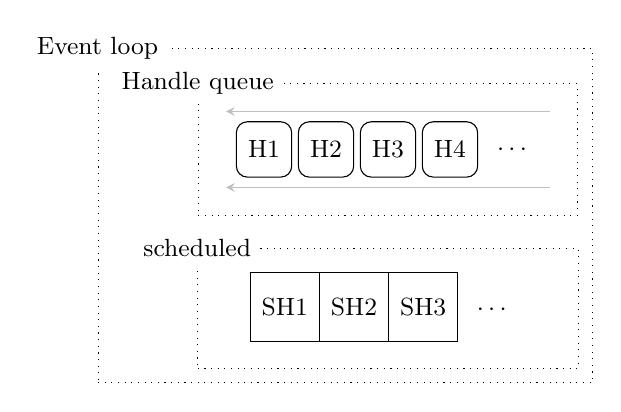
\begin{tikzpicture}[
    srrect/.style={rounded corners,minimum width=20pt,minimum height=20pt},
    sarr/.style={-stealth},font=\sffamily,font=\small,
    node distance=10pt
    ]
    \begin{scope}[start chain=going right,node distance=2pt,nodes={srrect,on chain}]
        \node[draw] (A2){H1};
        \node[draw] (B2){H2};
        \node[draw] (C2){H3};
        \node[draw] (D2){H4};
        \node[] (E2){$\cdots$};
    \end{scope}
    \node[fit=(A2) (E2)](F2){};
    \foreach \X in {north,south}
    {\draw[sarr,gray!50]  (F2.\X\space east) -- (F2.\X\space west);}
    \node[draw, fit=(F2), inner sep=10pt, dotted] (tq) {};
    \node[fill=white] (tqlabel) at (tq.north west) {Handle queue};
    \node[below=of tq, yshift=-20pt] (phan) {};
    \matrix[column sep=-\pgflinewidth, matrix of nodes, nodes={draw}, minimum size=25pt] (sh) at (phan.center) { SH1 & SH2 & SH3 & |[draw=none]|$\cdots$\\};
    \node[draw, dotted, fit= (sh) (tq.west |- phan.center) (tq.east |- phan.center), inner xsep=0pt, inner ysep=5pt] (shbox) {};
    \node[fill=white] (shlabel) at (shbox.north west) {scheduled};

    \node[draw, fit=(tq) (tqlabel) (shlabel) (shbox), inner sep=5pt, dotted] (eloop) {};
    \node[fill=white] (ellabel) at (eloop.north west) {Event loop};
\end{tikzpicture}

    \end{adjustbox}
    \end{center}
    {\ttfamily{Handle}} wraps \verb|Task.__step|
\end{frame}

\begin{frame}[plain, t]
    \frametitle{Task}
    \begin{center}
    \begin{adjustbox}{margin=10pt}
             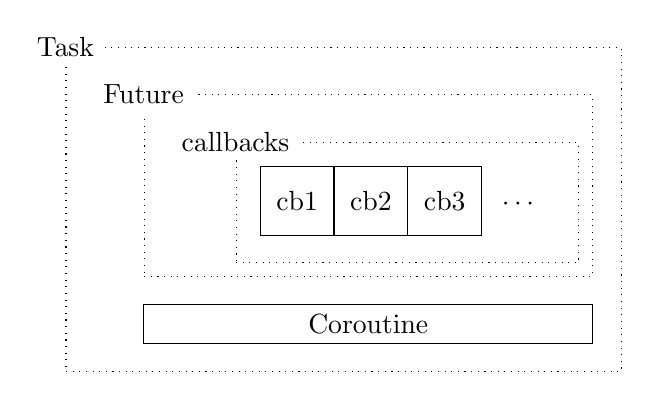
\begin{tikzpicture}[
array/.style={
    matrix of nodes,
    nodes={
        draw,
        text centered,
        text width=20pt,
        minimum size=25pt
    },
    column sep=-\pgflinewidth,
    nodes in empty cells,
    align=center,
    text centered
    },
    node distance=10pt
]

\matrix[array] (futcbarr) { cb1 & cb2 & cb3 &|[draw=none]|$\cdots$\\};
\node[draw, dotted, fit=(futcbarr), inner sep=5pt] (futcbbox) {};
\node[fill=white] (futcblabel) at (futcbbox.north west) {callbacks};
\node[draw, dotted, fit=(futcbarr) (futcblabel), inner sep=10pt] (futbox) {};
\node[fill=white] (futlabel) at (futbox.north west) {Future};
\node[below=of futbox] (coroboxcontent) {Coroutine};
\node[draw, inner sep=0, fit=(futbox.west |- coroboxcontent.center) (futbox.east |- coroboxcontent.center) (coroboxcontent)] (corobox) {};
\node[draw, dotted, fit=(corobox) (futbox) (futlabel), inner sep=10pt] (taskbox) {};
\node[fill=white] (tasklabel) at (taskbox.north west) {Task};

\end{tikzpicture}

    \end{adjustbox}
    \end{center}
\end{frame}

% \begin{frame}[plain, t, fragile]
%     \begin{lstlisting} 
%     def under__attack(col, queens):
%         left = right = col
%     \end{lstlisting}
% \end{frame}

\end{document}
